\chapter{Solving the Robust Optimal Guidance Problem}\label{Ch:SolutionMethod}
% UT transform to quantify mean/std of key variables
% Reformulation of the problem as a running cost and with a fixed independent variable 
% SLQ version of Differential Dynamic Programming algorithm for large scale solution 
% Analysis of necessary conditions??

Solving the robust optimal guidance problem presents a number of challenges. In this chapter we first discuss our choice of uncertainty quantification method used to compute the mean and standard deviation of key variables. Next we present the differential dynamic programming algorithm used to numerically solve the guidance problem. Finally, we detail several modifications to the problem to make it amenable to solution via DDP.

\section{Uncertainty Quantification}\label{Sec:UQ}
A key issue in solving the robust optimal guidance problem is computing the expected values and standard deviations in the objective functional and feedback terms. Broadly speaking, uncertainty quantification (UQ) methods trade between accuracy and the amount of computation required. For example, linear covariance propagation is one of the most efficient UQ methods for computing the first two probability moments, but its accuracy depends on the nonlinearity of the system dynamics. At the other extreme, Monte Carlo simulation can estimate higher order moments to arbitrary accuracy, but may require a huge number of samples in order to do so. Since UQ will be performed at each optimal control solver iteration, the method chosen must strike a careful balance these two aspects. For very fast but inaccurate methods, the solution may not perform as expected in a higher fidelity UQ, such as Monte Carlo simulation, and the benefit of the approach may be diminished or lost entirely. On the other hand, accurate methods will result in very long solution times. In this work, the unscented transform (UT) \cite{UT1997} is chosen to compute the required statistics. The following subsections review linear covariance and unscented transform methods. Then, via numerical example, we demonstrate that the saturation nonlinearity, introduced by the feedback control formulation Eq.~\eqref{Eq:Control}, is more accurately accounted for using the unscented transform. 

%The UT is preferable to linear covariance propagation in our application because the sigma points, described in a following subsection, are propagated through the full nonlinear, saturated dynamics, and are thus able to capture their effects on the distribution more accurately than linearization.

\subsection{Linear Covariance}
In the linear covariance methodology, the entry dynamics are linearized around a nominal state-control trajectory, and the mean trajectory is assumed to be equal to the nominal trajectory, i.e., $ \E{\state(v,\param)} \approx \state(v,\mathbf{0}) $. Compared with Eq.\eqref{Eq:TaylorExp}, we see this neglects a term related to the product of the covariance matrix and the trajectory curvature. 
The covariance matrix is propagated by integrating the Lyapunov differential equation
\begin{align}
	\dot{\cov}_{\state}(t) &= A(v)\cov_{\state}(v) + \cov_{\state}(v)A^T(v) \\
	A(v) &= \frac{\partial \dynamics_v}{\partial\state}\bigg\rvert_{x(v,\mathbf{0})}
\end{align}
subject to the initial condition $\cov_{\state}(v_0) = \cov_{\state_0}$. Note that the linearization around the nominal trajectory uses dynamics with respect to velocity, Eq.~\eqref{Eq:DynamicsWRTVel}. 
%TODO: clraify the notation, parameters are include in the state vector and thus the derivatives as well. 

\subsection{Unscented Transform}\label{Sub:UT}
The unscented transform is a method to approximate the first two moments of a nonlinear transformation of a probability distribution. Consider a scalar quantity $q\in\mathbb{R}$ resulting from a nonlinear transformation $q = F(\y)$ of a random vector $\y\in\mathbb{R}^n$ with known mean $ \bar{\y} $ and covariance $ \cov_{\y} $. A set of $2n+1$ sigma points and associated weights are computed 
\begin{align*}
	\y_0 &= \bar{\y} \\
	\y_i &=  \bar{\y} + \left(\sqrt{(\alpha+n) \cov_{\y}}\right)_i,\, \,i=1,...,n \\
	\y_{i+n} &=  \bar{\y} - \left(\sqrt{(\alpha+n)\cov_{\y}}\right)_i, \, \,i=1,...,n\\
	w_0 &= \frac{\alpha}{\alpha+n} \\
	w_i &= w_{i+n} = \frac{1}{2(\alpha+n)}, \, \,i=1,...,n
\end{align*}
where $\alpha$ is a scaling parameter, and $\left(\sqrt{(\alpha+n)\cov_{\y}}\right)_i$ is the $i^{\mathrm{th}}$ column of the matrix square root of $(\alpha+n) \cov_{\y}$. The sigma points are then mapped through the transformation
\begin{align}
	q_i = F(\y_i),\;\;i=0,...,2n
\end{align}
and finally, the mean and variance are estimated using the weights and transformed sigma points
\begin{align*}
	\bar{q} &\approx \sum_{i=0}^{2n}w_iq_i\\
	\sigma_{q} &\approx \left(\sum_{i=0}^{2n}w_i\left(q_i - \bar{q}\right)^2\right)^{\frac{1}{2}}
\end{align*}
In our application, $\y=\param$, the nonlinear transformation is the integration of the longitudinal entry dynamics to the terminal velocity, and the quantities of interest are downrange distance and altitude. For a given covariance matrix and a chosen value of $\alpha$, the ensemble of sigma points may be collected into a single extended vector, and the robust guidance problem is now a deterministic problem in the extended state space.
\begin{align}
	X = \begin{pmatrix}
	\state^{(0)}\\
	\vdots\\
	\state^{(2n)}
	\end{pmatrix}
\end{align}
When applying the unscented transform, the scaling parameter $\alpha$ is important in precisely estimating the statistics. For any value of $\alpha$, the sigma point distribution has the same mean and covariance as the initial distribution. Increasing the value of $\alpha$ places the sigma points $\y_i$ further from the nominal sigma point $\y_0$ and reduces their weight. Using a small value of $\alpha$ results in sigma points with only small deviations from the nominal, and for the entry guidance problem in this paper, the effects of the controller and saturation nonlinearity will not be accurately quantified. In our numerical studies, it appears that no single value of $\alpha$ minimizes estimation errors for all control profiles and all quantities of interest. However, it is important to recall that estimating statistics is not the purpose of the proposed trajectory optimization. So long as the reference trajectories designed using the UT confer benefits in Monte Carlo simulation, the UT statistics are sufficiently accurate, as will be demonstrated by the results of the numerical assessment. 

\subsection{Linear Covariance vs Unscented Transform Example}\label{Subsec:UQExample}
In this subsection we present a numerical example demonstrating the shortcoming of linear covariance propagation for our application to closed-loop entry guidance.
We simulate the performance of an MSL class entry vehicle using the feedback control, Eq.~\eqref{Eq:Control}. The example considers a single, non-optimized reference control and trajectory, and two sets of static feedback gains, $K_1=[0,0,0]^T$ and $K_2=[0.0725, -0.025, -0.004]^T$. $K_1$ corresponds to the open-loop case. The ballistic coefficient at the initial velocity is $\beta=120\,\mathrm{kg/m}^3$ and $L/D = 0.24$. The reference control is a linear-in-velocity ramp from 0.35 to 1. Additional details such as initial state and covariance are given in Chapter~\ref{Ch:AssessmentConditions}.
%TODO: finish giving the problem data,  uncertainties,

The terminal statistics are computed with three different UQ methods: linear covariance propagation (LC), unscented transform (UT), and Monte Carlo (MC). While the MC statistics are themselves estimates of the true mean and variance, accurate estimates can be by using a sufficiently large sample size. Thus they are the values against which statistics computed by LC and UT are compared. The UT scaling parameter $\alpha=15$ is used; sensitivity to this parameter is discussed below. Table~\ref{Table:UQCompareOpenLoop} presents the terminal statistics for the results using $K_1$; in this open-loop problem both LC and UT perform well. LC underestimates mean altitude by 1.2 km and altitude standard deviation by 200 m, underestimates mean range by 1 km, and overestimates range standard deviation by 1.1 km. In contrast, the UT overestimates the mean altitude by 160 m, the altitude standard deviation by 65 m, underestimates mean range by 800 m, and overestimates range standard deviation by 180 m. While the UT estimates a better in each variable, the LC estimates could be considered sufficient for the purposes of optimization. 

\begin{table}[h!]
	\centering
	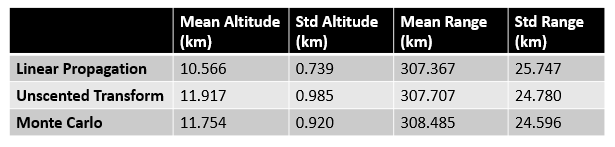
\includegraphics[width=1\textwidth]{Images/UQExample_Open}
	\caption{Comparison of UQ methods in an open-loop scenario}
	\label{Table:UQCompareOpenLoop}
\end{table}
\begin{table}[h!]
	\centering
	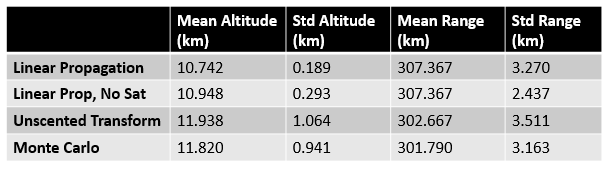
\includegraphics[width=1\textwidth]{Images/UQExample_Closed}
	\caption{Comparison of UQ methods in an closed-loop scenario}
	\label{Table:UQCompareClosedLoop}
\end{table}

Table~\ref{Table:UQCompareClosedLoop} presents the terminal statistics for the results using $K_2$. Linear propagation is listed twice; the first case linearizes the dynamics including the saturated controller defined in Eq.~\eqref{Eq:Control} while the second linearizes the controller without the saturation nonlinearity. In essence, the latter choice assumes the feedback control is not subject to the control limits, and as a result overpredicts the efficacy of the controller, as seen by the large underpredictions of the standard deviation of both altitude and range. Closed-loop robust optimal control was explored using linear sensitivity propagation without considering saturation in \cite{MarsEntryDesensitized}.
Both linearizations once again underpredict the mean altitude substantially. The UT overpredicts the mean range by 900 m and otherwise is once again accurate to within a few hundred meters or less for the remaining statistics. Note that this control profile has significant margin throughout the trajectory except close to the final velocity; in this case control saturation is likely not as significant as for reference control profiles that spend more time at or near the control limits. The UT is expected to produce greater benefits over LC in such scenarios.

\begin{figure}[h!]
	\centering
	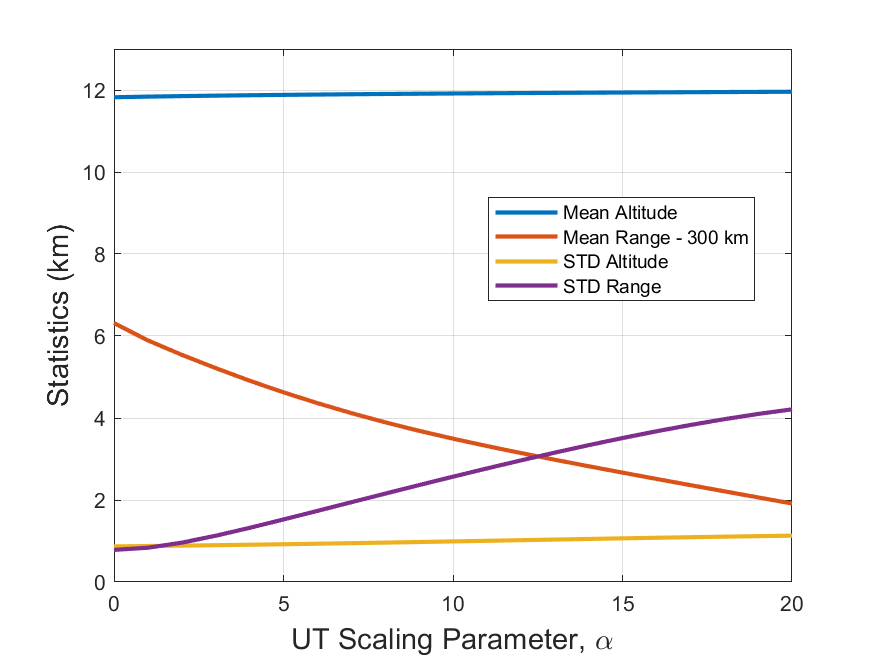
\includegraphics[width=1\textwidth]{Images/AlphaSensitivity}
	\caption{Sensitivity of statistics to the unscented transform scaling parameter}
	\label{Fig:AlphaSensitivity}
\end{figure}

Figure~\ref{Fig:AlphaSensitivity} shows how the UT-estimated means and standard deviations vary with different choices of the scaling parameter. Note that the mean range has been shifted down 300 km to fit it in the same figure. The altitude statistics are quite stable and vary only slightly with $\alpha$, while the effect is much stronger for range. This is a general phenomenon we have observed across numerous control profiles; as a result we recommend selection of $\alpha$ based on range considerations. 
Both the mean range and its standard deviation vary monotonically with $\alpha$. In this example, the mean range error is minimized for $\alpha = 20$, while $\sigma_s$ is approximately optimized for $\alpha = 13$. Our choice $\alpha=15$ strikes a balance between these two. 
While the tuning parameter $\alpha$ is important, we note that in this example the UT estimates of $\bar{h},\,\sigma_h$, and $\bar{s}$ are more accurate than either LC method for all of $\alpha$ values considered, and $\sigma_s$ is better for several values.
This example is meant to motivate our choice of the UT over LC; more detailed examples utilizing optimal solutions are presented in Chapter~\ref{Ch:NumericalAssessment}. 
%TODO: Show control profile, trajectory plots with MC samples, UT points? Or maybe just estimated 3-sigma bounds but might be too messy with three on there Also show a table of the terminal statistics. 

%Sensitivity to $\alpha$  
%Talk about the (weak) dependence on alpha, such that we can choose a single decent value and use it for all of the solutions? 

\section{Differential Dynamic Programming}\label{Sec:DDP}
We begin this section by reviewing the control-limited differential dynamic programming method, proposed in Ref.~\cite{DDP_ControlLimited}, that will be used as the basis for solving the robust optimal guidance problem. The following subsections discuss modifications to the algorithm and the problem formulation that will finally enable the solution of the problem. In the first subsection we present a extension of the algorithm that allows for the joint optimization of static design parameters. The following subsection proposes a simplification that vastly reduces computational time and memory requirements at the expense of lower convergence rate. This simplification is instrumental in solving the large-scale problem. Next, we discuss a reformulation of the performance objective into a Lagrange (or running) cost instead of a Mayer (or terminal) cost. Finally, we present a differentiable approximation to the saturation nonlinearity in the controller, Eq.~\eqref{Eq:Control}. Since DDP requires derivatives of the dynamic equations with respect to the reference control, state variables, and potentially the feedback gains, replacing the non-differentiable saturation function is essential to the numerical solution.

DDP is a trajectory optimization method that iteratively solves for a locally optimal trajectory and control starting from a nominal trajectory and control.

This particular DDP algorithm is formulated in discrete time, so the continuous time dynamics must be discretized. In our numerical examples, Euler integration is used:
\begin{align}
	\state_{i+1} = \mathbf{f}(v, \state_i,\control_i) = \state_i + \state_i'\Delta v \label{Eq:DiscreteDynamics}
\end{align}
A trajectory $\{\State,\Control\}$ is a sequence of controls $ \Control=\{\control_0,\control_1,...,\control_{N-1}\} $ and corresponding states $\State=\{\state_0,\state_1,...,\state_N\}$ determined by integrating \eqref{Eq:DiscreteDynamics} from $\state_0$.
Although the optimal control objective as posed considers only a terminal cost, in this section we consider a generic cost function $J$ consisting of a sum of running costs $l$ and a terminal cost $l_N$:
\begin{align}
	J(\state_0,\Control) = \sum_{i=0}^{N-1}l(\state_i,\control_i) + l_N(\state_N)
\end{align}
Let $\Control_i$ be the tail of the control sequence, $\{\control_i,\control_{i+1},...,\control_{N-1}\}$, and the cost-to-go $J_i$, defined as the partial sum of costs from $i$ to $N$ is
\begin{align}
	J_i(\state,\Control_i) = \sum_{j=i}^{N-1}l(\state_j,\control_j) + l_N(\state_N)
\end{align}
The value function at timestep $i$ is the optimal cost-to-go at \state
\begin{align}
	V_i(\state) = \min_{\Control_i} J(\state, \Control_i)
\end{align}
and at the final timestep the value function is equal to the terminal objective. The dynamic programming principle reduces the problem of minimization over $\Control_i$ to a sequence of minimization problems over $u$ at each timestep 
\begin{align}
	V(\state) = \min_{\control}\left[l(\state,\control) + V^+(\mathbf{f}(\state,\control))\right] \label{eq_dynamic_programming}
\end{align}
where $V^+$ is the value at the next time step.
Let the pseudo-Hamiltonian $Q(\delta\state,\delta\control)$ be the change in value function as a function of perturbations to the pair $(\state,\control)$:
\begin{align}
	Q(\delta\state,\delta\control) = l(\state+\delta\state,\control+\delta\control) + V^+(\mathbf{f}(\state+\delta\state,\control+\delta\control))
\end{align}
The second-order expansion of $ Q $ is given by
\begin{align}
	Q_\state &= l_\state + \mathbf{f}_\state^T V^+_\state \\
	Q_\control &= l_\control + \mathbf{f}_\control^T V^+_\state \\
	Q_{\state\state} &= l_{\state\state} + \mathbf{f}_\state^T V^+_{\state\state}\mathbf{f}_\state + V^+_\state \mathbf{f}_{\state\state} \label{eq_hessian1}\\
	Q_{\control\state} &= l_{\control\state} + \mathbf{f}_\control^T V^+_{\state\state}\mathbf{f}_\state + V^+_\state \mathbf{f}_{\control\state} \label{eq_hessian2}\\
	Q_{\control\control} &= l_{\control\control} + \mathbf{f}_\control^T V^+_{\state\state}\mathbf{f}_\control + V^+_\state \mathbf{f}_{\control\control} +\lambda I \label{eq_hessian3}
\end{align}
where the subscripts denote partial derivatives with respect to that quantity, and the final term in each of the Hessian equations (\ref{eq_hessian1})-(\ref{eq_hessian3}) are tensor-vector contractions, and $ \lambda $ is a regularization parameter.  %TODO: rewrite them as sums over the 'pages' of the hessian

The optimal control modification $\delta\control^*$ for some perturbation $\delta\state$ is a locally-linear feedback control $\delta\control^* = \mathbf{k} + K\delta\state$ obtained by minimizing the quadratic model subject to linear bounds on the controls
\begin{align}
	\mathbf{k} = &\arg\min_{\delta\control} Q(\delta\state,\delta\control) \\
	&\mathrm{subject\,to\,\;} \nonumber\\
	\control_{\min}\le &\control+\delta\control \le\control_{\max}
\end{align}
and $K = -Q_{\control\control}^{-1}Q_{\control\state}$. Substituting the optimal control into the expansion of $Q$, a quadratic model of $V$ is obtained with derivatives
\begin{align}
	\begin{split}
		\label{eq_value_recurse}
		V_\state &= Q_{\state}- K^TQ_{\control\control}\mathbf{k}\\
		V_{\state\state} &= Q_{\state\state} - K^TQ_{\control\control}K.
	\end{split}
\end{align}
The backward pass is performed by initializing $V$ and its derivatives with the value and derivatives of the terminal objective, then recursively computing the optimal control policy and Eq.~(\ref{eq_value_recurse}). 

The forward pass uses the newly computed control policy to integrate the new trajectory, subject to a backtracking line search
\begin{align}
	\hat{\state}_0 &= \state_0 \\
	\hat{\control}_{i} &= \control_i + \epsilon \mathbf{k}_i + K_i(\hat{\state}_i - \state_i)\\
	\hat{\state}_0 &= f(\hat{\state}_i,\hat{\control}_i)
\end{align}
where $\epsilon$ is a search parameter initialized to 1 and reduced until the value function shows improvement. The backward-forward iterations are repeated until convergence to a locally optimal trajectory. In the event the backward pass fails to produce a descent direction, the regularization parameter $\lambda$ is increased and the backward pass is repeated. See Ref.~\cite{DDP_ControlLimited} for more details about the line search and regularization procedures. 

%TODO: maybe move this into the DDP section and discussion from the start? Call it a modification to treat the EFPA, that can also be used for other constant design parameters by appending them to the state? Hard to justift that approach when Im not optimizing the EFPA though 
\subsection{Optimal Design Parameters}\label{Sec:DesignOptimization}
Previously, we considered the state vector to be a function of the independent variable and the uncertainty vector $\param$. However, we may wish to treat the state as a function of some additional constant design parameters, $\design$, $\state(v, \param, \design)$. The design parameters are different from the uncertain parameters because they do not increase the number of sigma points required. Additionally, in our formulation, the design parameters are appended only to the extended vector of all sigma points. Thus, given state dimension $n_x$, uncertainty dimension $n_p$, and design parameter dimension $n_d$, the total number of states is $n_x(2n_p+1) + n_d$. We define an augmented state vector $\state_a = [\xut, \design]^T$ 
and augment the entry dynamics with trivial dynamics
\begin{align}
	\state_a' = \left[
	\begin{matrix}
		\xut' \\
		\mathbf{0}
	\end{matrix}
	\right]
\end{align}
DDP is now applied to the augmented state vector with an additional modification that we will explain. In \cite{DDP:ContinuousTerminalConstraints}, Lagrange multipliers are used to enforce terminal constraints in a continuous time DDP formulation. At the end of each backward pass, the Lagrange multipliers are updated to reduce the cost function. Although the setting was quite different, we notice that the form of the update to the Lagrange multipliers actually applies to any constant parameter and is the inspiration for our proposed modification to the discrete time algorithm.

During the backward pass, the first and second partial derivatives of the value function are computed recursively from the final velocity to the initial velocity. The gradient and hessian of the value function can be written in block notation as 
\begin{align}
	V_{\state_a} &= \begin{bmatrix}
		V_\state & V_\design
	\end{bmatrix} \\
	V_{\state_a\state_a} &= \begin{bmatrix}
		V_{\state\state} & V_{\state\design} \\
		V_{\design\state} & V_{\design\design}
	\end{bmatrix}
\end{align}
The quadratic expansion of the value function at the initial velocity is
\begin{align}
	V(v_0, \state_a+\delta\state_a) = V(v_0, \state_a) + V_{\state_a}^T\delta_{\state_a} + \frac{1}{2}\delta_{\state_a}^TV_{\state_a\state_a}\delta_{\state_a} \label{Eq:ValueExpansion}
\end{align}
At the end of the backward pass, we set $\delta\state_a=\zero$ because we are optimizing a trajectory from a fixed initial state. However, when including design parameters that can be altered, we can derive an update $\delta\state_a = [\zero,\delta\design]^T$ to reduce the value function based on the expansion \eqref{Eq:ValueExpansion}, which simplifies to 
\begin{align}
	V(v_0, \design+\delta\design) = V(v_0, \design) + V_{\design}^T\delta_{\design} + \frac{1}{2}\delta_{\design}^TV_{\design\design}\delta_{\design} \label{Eq:ValueParamExpansion}
\end{align}
The $\delta_{\design}$ that minimizes Eq.~\eqref{Eq:ValueParamExpansion} is determined by the solution to $V_{\design} + V_{\design\design}\delta_{\design} = 0$, or 
\begin{align}
	\delta_{\design} = -V_{\design\design}^{-1}V_{\design}
\end{align}
In practice, the update must be treated like the control updates by using a line search $\delta_{\design} = -\epsilon_{\design} V_{\design\design}^{-1}V_{\design}$. While a different line search parameter could be utilized, in our implementation we take $\epsilon_\design=\epsilon$. There is no guarantee that $V_{\design\design}$ is positive definite, and thus regularization of the matrix may be required. Unlike the control regularization, which uses a single value for the entire backward pass and is iteratively updated, the design regularization is computed only once per backward pass, and the number of design parameters in generally small. For this reason, the regularization method preferred here is to compute the eigenvalues of $V_{\design\design}$, and replace small/negative eigenvalues with regularization term - shifting from Newton-like to gradient descent as the amount of regularization increases.

%This can be used to jointly optimize the feedback gains, entry flight path angle and more. This is motivated by the ``overfitting" problem. 

\subsection{Second Order Dynamics Derivatives}\label{Sec:DDP_Simplification}
%TODO: Show an example with and without the second order terms to compare convergence. Either here, or maybe in the numerical assessment section. 
The second derivatives $\mathbf{f}_{\state\state},\, \mathbf{f}_{\control\state}$ in Eqs.~\eqref{eq_hessian1})~and~\eqref{eq_hessian2} are $n\times n\times n$ and $m\times n\times n$ tensors, respectively, that must either be stored at $N$ timesteps, or else recomputed in the event the backward pass must be repeated with increased regularization. For large $n$, both computing and storing these quantities is problematic. Unfortunately, removing these terms entirely, as is done in the iterative Linear Quadratic Gaussian method \cite{iLQG}, leads to poor performance for the problem under consideration. In particular, the first-order algorithm has a noticeably smaller radius of convergence, and different guesses at the initial control sequence often lead to different local minima. In contrast, the full second-order DDP algorithm consistently converges to a single minimum from most initial guesses. Thus, we propose a compromise in which only the $n\times m \times m$ tensor $f_{\control\control}$ is retained in the above equations. Numerical experiments suggest this is sufficient to avoid poor solutions, at the expense of a slower convergence rate than the full algorithm with all second-order terms included. However, in the situation at hand, in which the number of controls $m$ is fixed and small ($ m=1 $), and the augmented state dimension, which depends on the number of uncertainties under consideration, is large ($n=78$ for $\param\in\mathbb{R}^6$), this modification proves to be enabling for $N\geq 100$. A limited-memory version of the Quasi-Newton approximations to these terms proposed in \cite{QNDDP} may also be a good choice to obtain superlinear convergence properties of the approximated second-order algorithm while reducing the memory required. 
%(This reduces complexity from cubic in $n$ to linear)

\subsection{Objective Reformulation}
In order for DDP to be applied to our robust optimal control problem, it is essential to reformulate some or all of the objective terms as running costs rather than terminal costs. This is because the terminal formulation results in singularity of the Hessian of the pseudo-Hamiltonian with respect to the control, and this quantity must be invertible for the algorithm to proceed. 
%In practice, one could also add a small control regularization term to the objective, but experience indicates that reformulating the mean altitude objective is preferable. 
The reformulation is based on the relationship 
\begin{align}
	J(\state(v_f)) = J(\state_0) + \int_{v_0}^{v_f}J'\mathrm{d}v \label{Eq:GenericCostRate}
\end{align}
For a fixed initial state, the term $J(\state_0)$ is constant and cannot be affected by the control profile. As such, 
\begin{align}
	u^* &= \arg\min \,J(\state(v_f)) \\
	&= \arg\min\int_{v_0}^{v_f}J'\mathrm{d}v
\end{align}
Thus, we need an expression for $J'$ for the guidance objective defined in Eq.~\eqref{Eq:Objective}. Due to linearity of the expectation operator, we have the following relationships for the rate of change of the first two moments of a scalar random variable
%\begin{align}
%\frac{d }{d t}\E{x} &= \E{\dot{x}} \label{Eq:MeanRate}\\
%\frac{d }{d t}\V{x} &= \E{2x\dot{x}} - 2\E{x}\E{\dot{x}} \\
%\sigma_x &= \V{x}^{\frac{1}{2}} \\
%\frac{d }{d t}\sigma_x &= \frac{1}{2\sigma_x}\frac{d }{d t}\V{x} \\
% &= \frac{1}{\sigma_x}\left(\E{x\dot{x}} - \E{x}\E{\dot{x}}\right) \label{Eq:StdRate}
%\end{align}
%Equations~\eqref{Eq:MeanRate} and \eqref{Eq:StdRate} are converted into velocity rates
\begin{align}
	\frac{d }{d v}\E{x} &= \E{x'} \label{Eq:MeanRateVel}\\
	\frac{d }{d v}\V{x} &= \E{2xx'} - 2\E{x}\E{x'} \\
	\sigma_x &= \V{x}^{\frac{1}{2}} \\
	\frac{d }{d v}\sigma_x &= \frac{1}{\sigma_x}\left(\E{xx'} - \E{x}\E{x'}\right) \label{Eq:StdRateVel}
	%\frac{d }{d t}\V{x}^{\frac{1}{2}} &= \frac{1}{2\V{x}^{\frac{1}{2}}}\frac{d }{d t}\V{x}
\end{align}
Applying these to altitude and downrange distance, and discretizing the resulting integral, we arrive at the 
the reformulated discrete-time running cost
\begin{align}
	%J = \int_{v_0}^{v_f}-\E{h'} +  2w_h(\E{hh'}-\E{h}\E{h'}) + 2w_s(\E{ss'}-\E{s}\E{s'})\mathrm{d}v \\
	%J = \sum_{i=0}^{N-1} \left[-\E{h'} +  2w_h(\E{hh'}-\E{h}\E{h'}) + 2w_s(\E{ss'}-\E{s}\E{s'})\right]\delta v 
	l(\state,\control) = \left(-\E{h'} +  \frac{w_h}{\sigma_h}(\E{hh'}-\E{h}\E{h'}) + \frac{w_s}{\sigma_s}(\E{ss'}-\E{s}\E{s'})\right)\Delta v
\end{align}
While reformulating the mean altitude objective is essential to solving the problem, especially when $w_s=w_h=0$, reformulating the standard deviation terms is not. However, in numerical experiments we found that while both formulations result in the same solution, using running costs for the standard deviations allows DDP to converge in noticeably fewer iteration. Running costs are used in the results in this dissertation.

\subsection{Saturation}
The saturation function in Eq.~\eqref{Eq:Control} is not differentiable at the  saturation limits, which produces numerical difficulties for the DDP algorithm. To circumvent this problem, we substitute the following smooth approximation when solving the robust optimal guidance problem
\begin{align*}
	\mathrm{sat}_{[0,1]}(x) \approx \frac{1}{2} + \frac{1}{4M}\log\left(\frac{\cosh (2Mx)}{\cosh (2M(x-1))}\right) 
\end{align*}
where $M>0$ is a tuning parameter. Larger values of $M$ reduce approximation error but increase the derivative magnitude at the saturation limits. $M=20$ reduces the maximum error to less than $1\%$ and is used in our implementation. Figure~\ref{Fig:SmoothSat} shows how the approximation varies with $M$; at $M=20$, the approximation is visually indistinguishable from the true function.
\begin{figure}[h!]
	\centering
	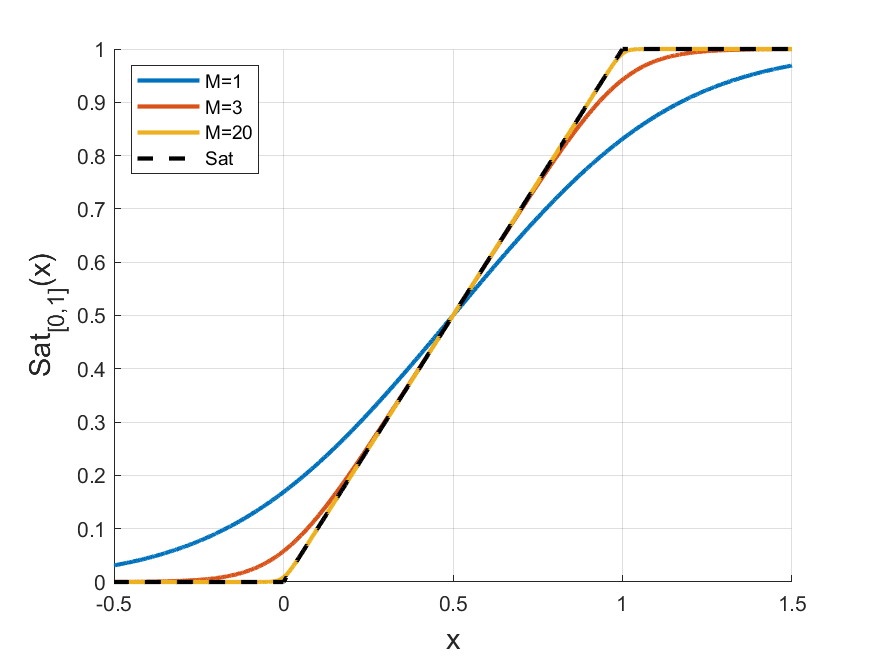
\includegraphics[width=1\textwidth]{Images/SmoothSat}
	\caption{The saturation function and smooth approximation for several values of the tuning parameter.}
	\label{Fig:SmoothSat}
\end{figure}



%\section{UT-Approximated Robust Guidance Problem}
%Let \xut = 
%\begin{align}
%	&\min J = -\bar{h}(v_f) + w_h\sigma_h(v_f) + w_s\sigma_s(v_f) \nonumber\\
%	&\quad\quad\qquad\mathrm{subject\, to }\nonumber \\
%	&\dot{\xl}(v,\param) = \dynamics_v(v, \xl(v,\param), u(v), \param),\quad
%	\xl(v_0,\param) = \state_0(\param) \nonumber\\
%	&\param\sim \normal(\mathbf{0},\cov_{\param}) \nonumber\\
%	&0 \le \ur(v) \le 1 \quad \forall\,v\in [v_0, v_f] \nonumber
%\end{align}

%\section{Necessary Conditions}
%In this section the necessary conditions for an optimal solution to the robust optimal guidance problem are given. Since the terminal objective function has been reformulated as a Lagrange (or running) cost
%\begin{align}
%	J = \int_{v_0}^{v_f}\left[ -\E{h'} +  \frac{w_h}{\sigma_h}(\E{hh'}-\E{h}\E{h'}) + \frac{w_s}{\sigma_s}(\E{ss'}-\E{s}\E{s'})\right]\, \mathrm{d}v
%\end{align}
%and thus the Lagrange cost is
%\begin{align}
%	L(x,u) =  -\E{h'} +  \frac{w_h}{\sigma_h}(\E{hh'}-\E{h}\E{h'}) + \frac{w_s}{\sigma_s}(\E{ss'}-\E{s}\E{s'})
%\end{align}
%The UT approximation of $L$ is given by
%\begin{align}
%	L_{UT}(x,u) =  -\EUT{h'} +  \frac{w_h}{\sigma_h}(\EUT{hh'}-\EUT{h}\EUT{h'}) + \frac{w_s}{\sigma_s}(\EUT{ss'}-\EUT{s}\EUT{s'})
%\end{align}
%
%The Hamiltonian for the UT-approximated ROCP is 
%$H = \lambda^Tf(v,\state(v),\param)+ L(\state,\param)$ 


%%% Local Variables: ***
%%% mode: latex ***
%%% TeX-master: "thesis.tex" ***
%%% End: ***
